\documentclass[letterpaper, 12pt]{report}
\usepackage[utf8]{inputenc}
\usepackage[english, spanish]{babel}
\usepackage{fullpage} % changes the margin
\usepackage{graphicx}
\usepackage{enumitem}
\usepackage{chngcntr}
\usepackage{multirow}
\usepackage{parskip}
\counterwithin{figure}{section}
\renewcommand{\thesection}{\arabic{section}}
\renewcommand{\thesubsection}{\thesection.\arabic{subsection}}
\renewcommand{\baselinestretch}{1.5}
\usepackage{float}
\bibliographystyle{apalike}
\setlength\belowcaptionskip{10pt}
\linespread{1.5}

\raggedbottom{}

\begin{document}

\begin{titlepage}
	\centering
	
\includegraphics[width=0.3\textwidth]{Images/logo_utb.png}\par\vspace{1cm}
	{\scshape\LARGE Universidad Tecnológica de Bolívar \par}
	\vspace{1cm}

	{\scshape\Large FÍSICA ELÉCTRICA \par}
	\vspace{.2cm}

	% chktex-file 8
	{\scshape\Large H1 - C \par}
	\vspace{1cm}
	% chktex-file 8
	\slshape {\Large \bfseries{}Informe de Laboratorio No. 3 \\}
	\vspace{1cm}

	\slshape {\itshape{} Mauro González, T00067622 \\}
	\slshape {\itshape{} German De Armas Castaño, T00068765 \\}
	\slshape {\itshape{} Angel Vega Rodriguez, T00068186 \\}
	\slshape {\itshape{} Juan Jose Osorio Ariza, T00067316 \\}
	\slshape {\itshape{} Juan Eduardo barón, T00065901 \\}
	\vfill
	Revisado Por \\
	Gabriel Hoyos Gomez Casseres\\
	{\large \today\par}
\end{titlepage}

% ----------------------------------------------------------------------|>
\section{Introducción}

Las superficies equipotenciales y las líneas de campo eléctrico son conceptos
fundamentales en el estudio de la electricidad y el magnetismo.

\vspace{.5cm}

En el desarrollo de esta práctica se busca comprender el comportamiento de
la energía eléctrica en un sistema controlado, para evidenciar en su plenitud
el fenómeno conocido como una superficie equipotencial, que consiste en una
superficie tridimensional en la cual el potencial eléctrico es constante en
todos sus puntos. En otras palabras, cualquier punto en una superficie
equipotencial tiene el mismo potencial eléctrico.

\vspace{.5cm}

Por otro lado, las líneas de campo eléctrico son líneas
imaginarias que se dibujan en el espacio para representar
la dirección y la intensidad del campo eléctrico.

\vspace{.5cm}

Las líneas de campo eléctrico son siempre perpendiculares a las
superficies equipotenciales y apuntan en la dirección en la que una
carga positiva se movería si se colocara en el campo eléctrico.
En conjunto, las superficies equipotenciales y las líneas de campo eléctrico
nos permiten visualizar y comprender el comportamiento de los campos eléctricos
en diferentes situaciones. Además, nos permiten calcular el trabajo
necesario para mover una carga en el campo eléctrico y la dirección en
la que se moverá la carga. Estos conceptos son fundamentales para la
comprensión de fenómenos como la electrostática, la capacitancia y la
conductividad eléctrica.

\newpage

% ----------------------------------------------------------------------|>
\section{Objetivos}

\subsection{Objetivo General}

Analizar con cada tipo de  electrodo los diferentes comportamientos de las
lineas de campo eléctrico.

\subsection*{Objetivos específicos}

\begin{itemize}
	\item Analizar las características de las lineas equipotenciales y de
	      campo eléctrico.
	\item Comprender la relación existente entre campo eléctrico y potencial
	      eléctrico
	\item Utilizar las coordenadas en el campo cartesiano para dibujar las
	      lineas de campo eléctrico a través de las lineas equipotenciales
\end{itemize}

\newpage

% ----------------------------------------------------------------------|>
\section{Marco Teórico}

\subsection{Superficies equipotenciales}

Es una superficie tridimensional sobre la que el potencial
eléctrico V es el mismo en todos los puntos. Si una carga de prueba q0 se 
desplaza de un punto a otro sobre tal superficie, la energía potencial 
eléctrica q0 V permanece constante. En una región en la que existe un campo 
eléctrico es posible construir una superficie equipotencial a través de 
cualquier punto.

\begin{figure}[H]
	\begin{center}
		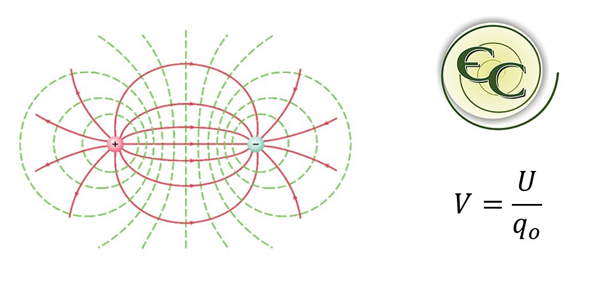
\includegraphics[scale = 1]{./Images/Equipotenciales.png}
		\caption{Superficies equipotenciales}
	\end{center}
\end{figure}

En toda superficie equipotencial, el potencial es constante, en consecuencia,
para un desplazamiento sobre una superficie lo que indica que el campo
eléctrico en la dirección tangencial a la superficie es cero. Por consiguiente, 
el campo eléctrico debe ser totalmente perpendicular a la superficie.
\textit{(Universidad del valle Colombia, Las Lineas equipotenciales las super 
- lineas equipotenciales)}

\vspace{1.5cm}

Para realizar este cálculo usamos la ley de coulomb, esta nos describe la 
interacción que  tienen dos cargas con mismo o diferente signo. 
La fuerza que ejerce la carga Q sobre otra carga q situada en una distancia r 
está dada por la formula:

\begin{figure}[H]
	\begin{center}
		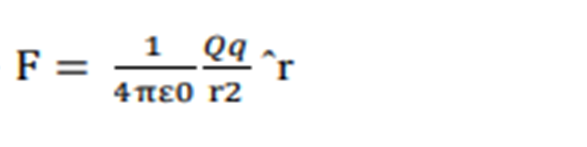
\includegraphics[scale = 1]{./Images/FormulaCoulumb.png}
	\end{center}
\end{figure}

El radio (r) determina el potencial, por lo tanto, las líneas equipotenciales son 
círculos y superficie de una esfera centrada sobre la carga de una superficie.

\subsection{Lineas Equipotenciales}

Las líneas de campo y las superficies equipotenciales siempre son 
perpendiculares entre sí. En general, las líneas de campo son curvas, y 
las equipotenciales son superficies curvas. Para el caso especial de un campo 
uniforme, en el que las líneas de campo son rectas, paralelas y están 
igualmente espaciadas, las superficies equipotenciales son planos paralelos 
perpendiculares a las líneas de campo.~\cite{blas_fernandez}


% ----------------------------------------------------------------------|>
\section{Montaje Experimental}

\begin{figure}[H]
	\begin{center}
		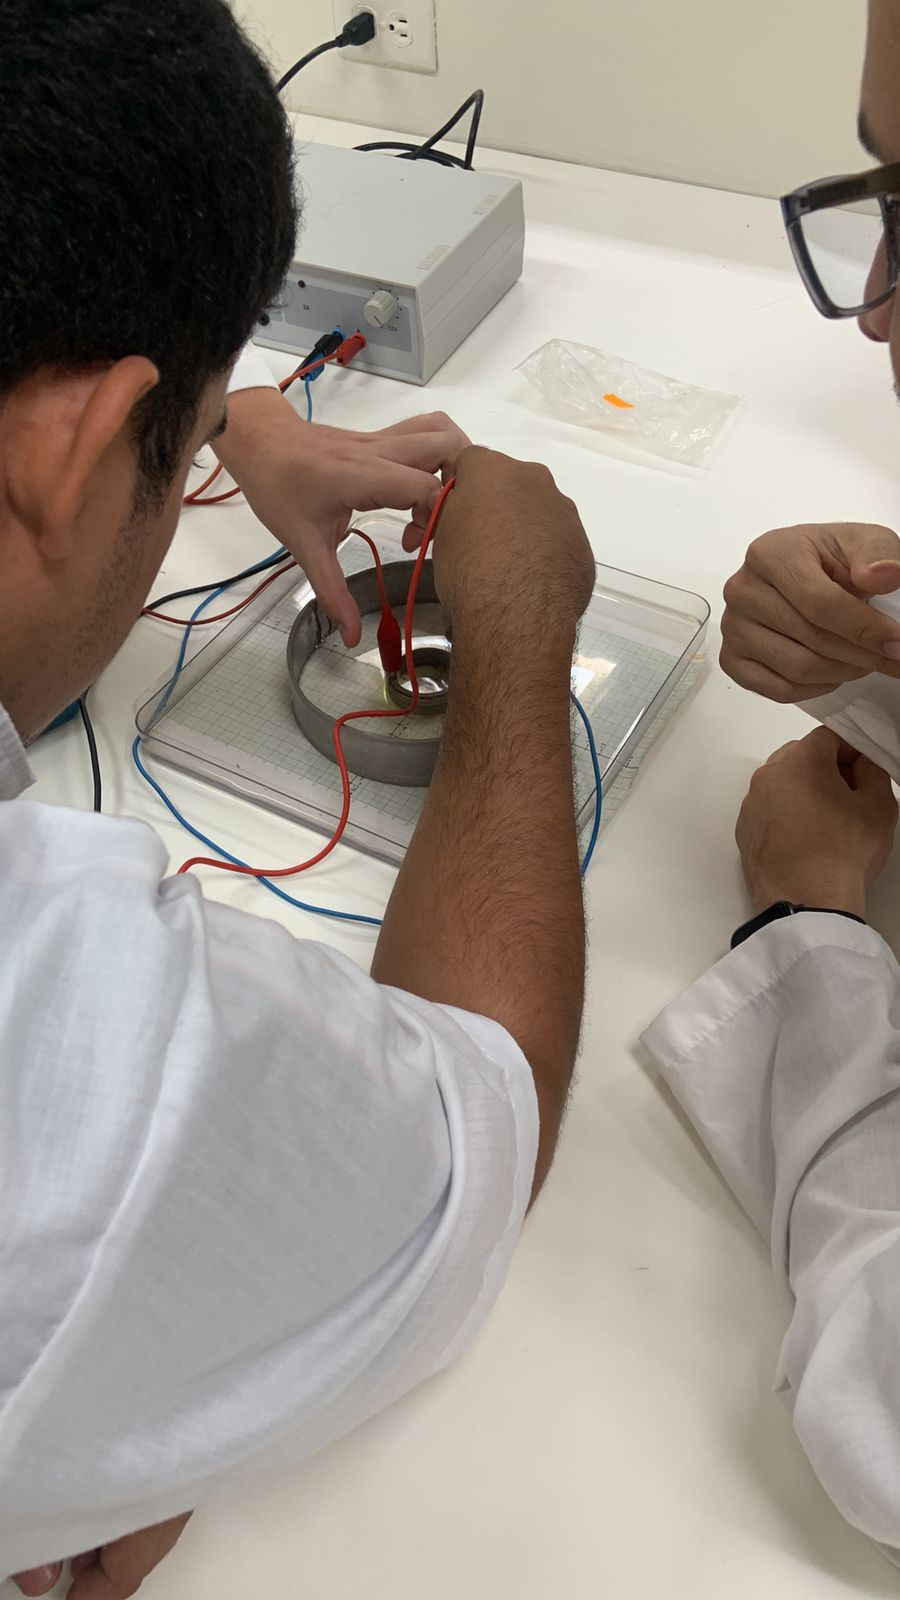
\includegraphics[scale = 0.3]{./Images/1.jpeg}
		\caption{Montaje electrodos concéntricos (1)}
	\end{center}
\end{figure}

\begin{figure}[H]
	\begin{center}
		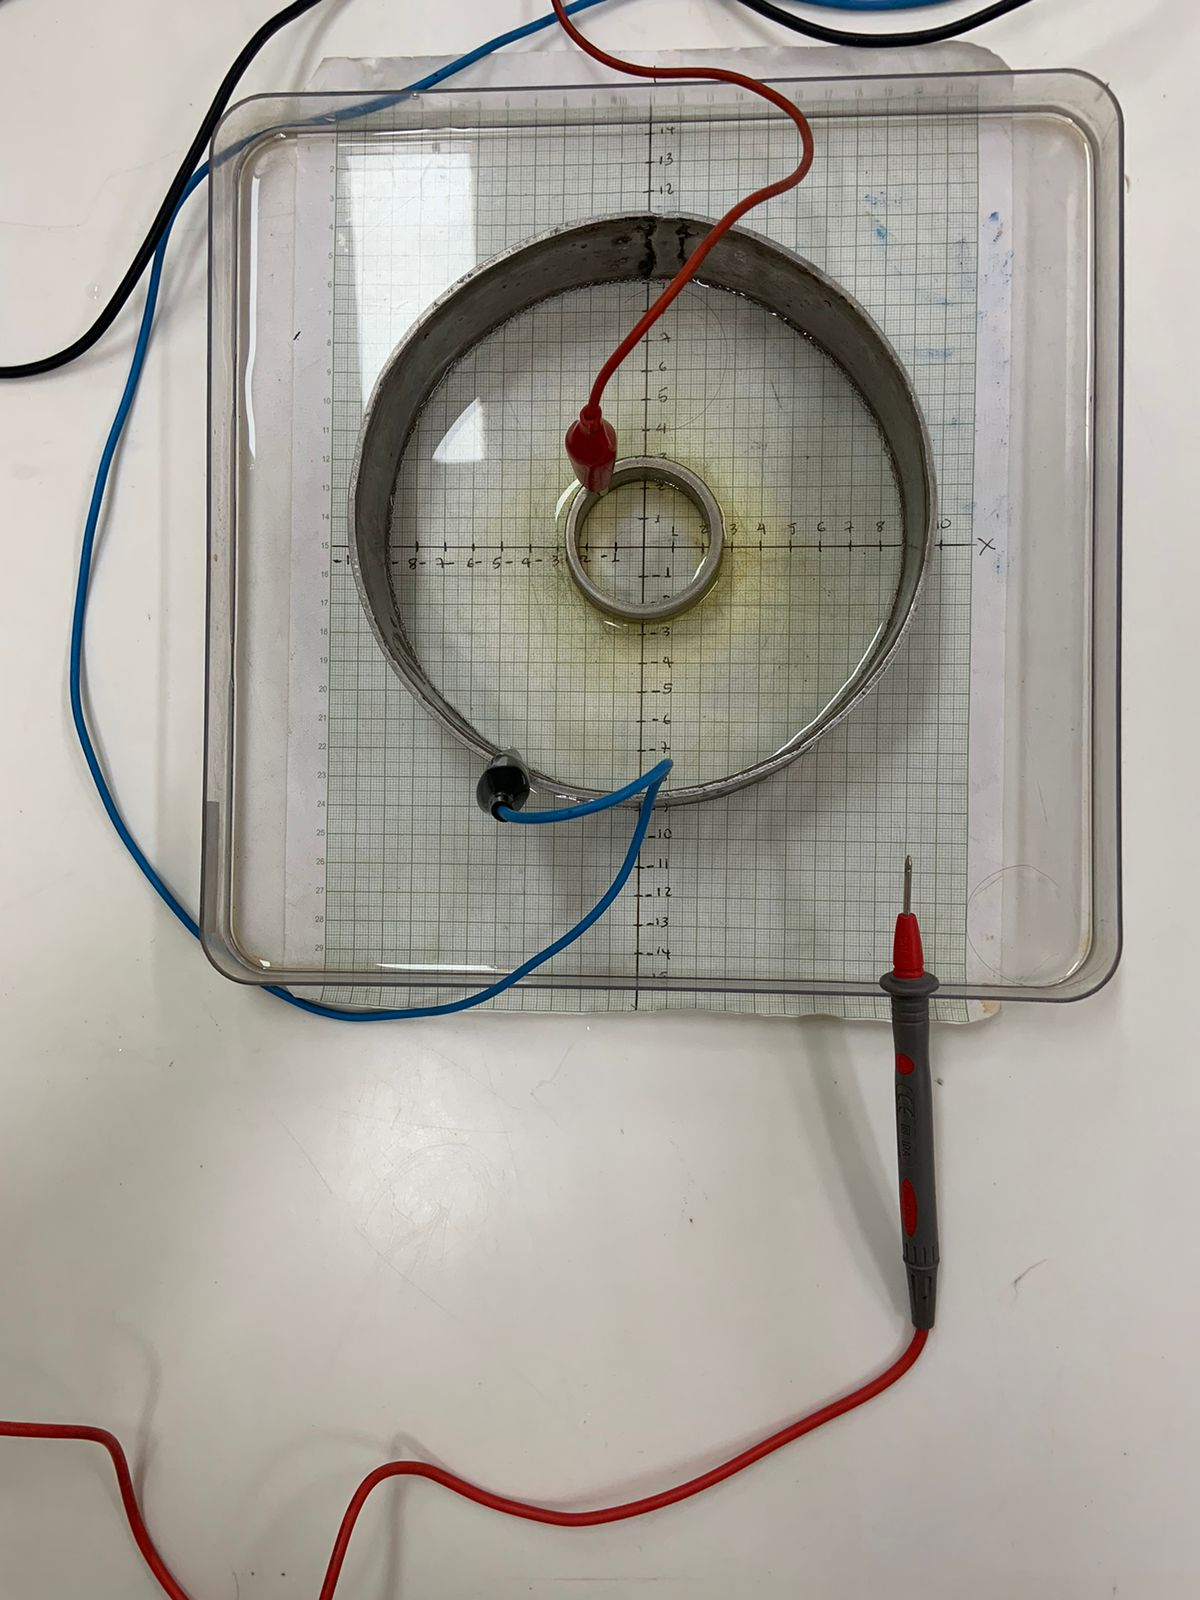
\includegraphics[scale = 0.3]{./Images/2.jpeg}
		\caption{Montaje electrodos concéntricos (2)}
	\end{center}
\end{figure}

\begin{figure}[H]
	\begin{center}
		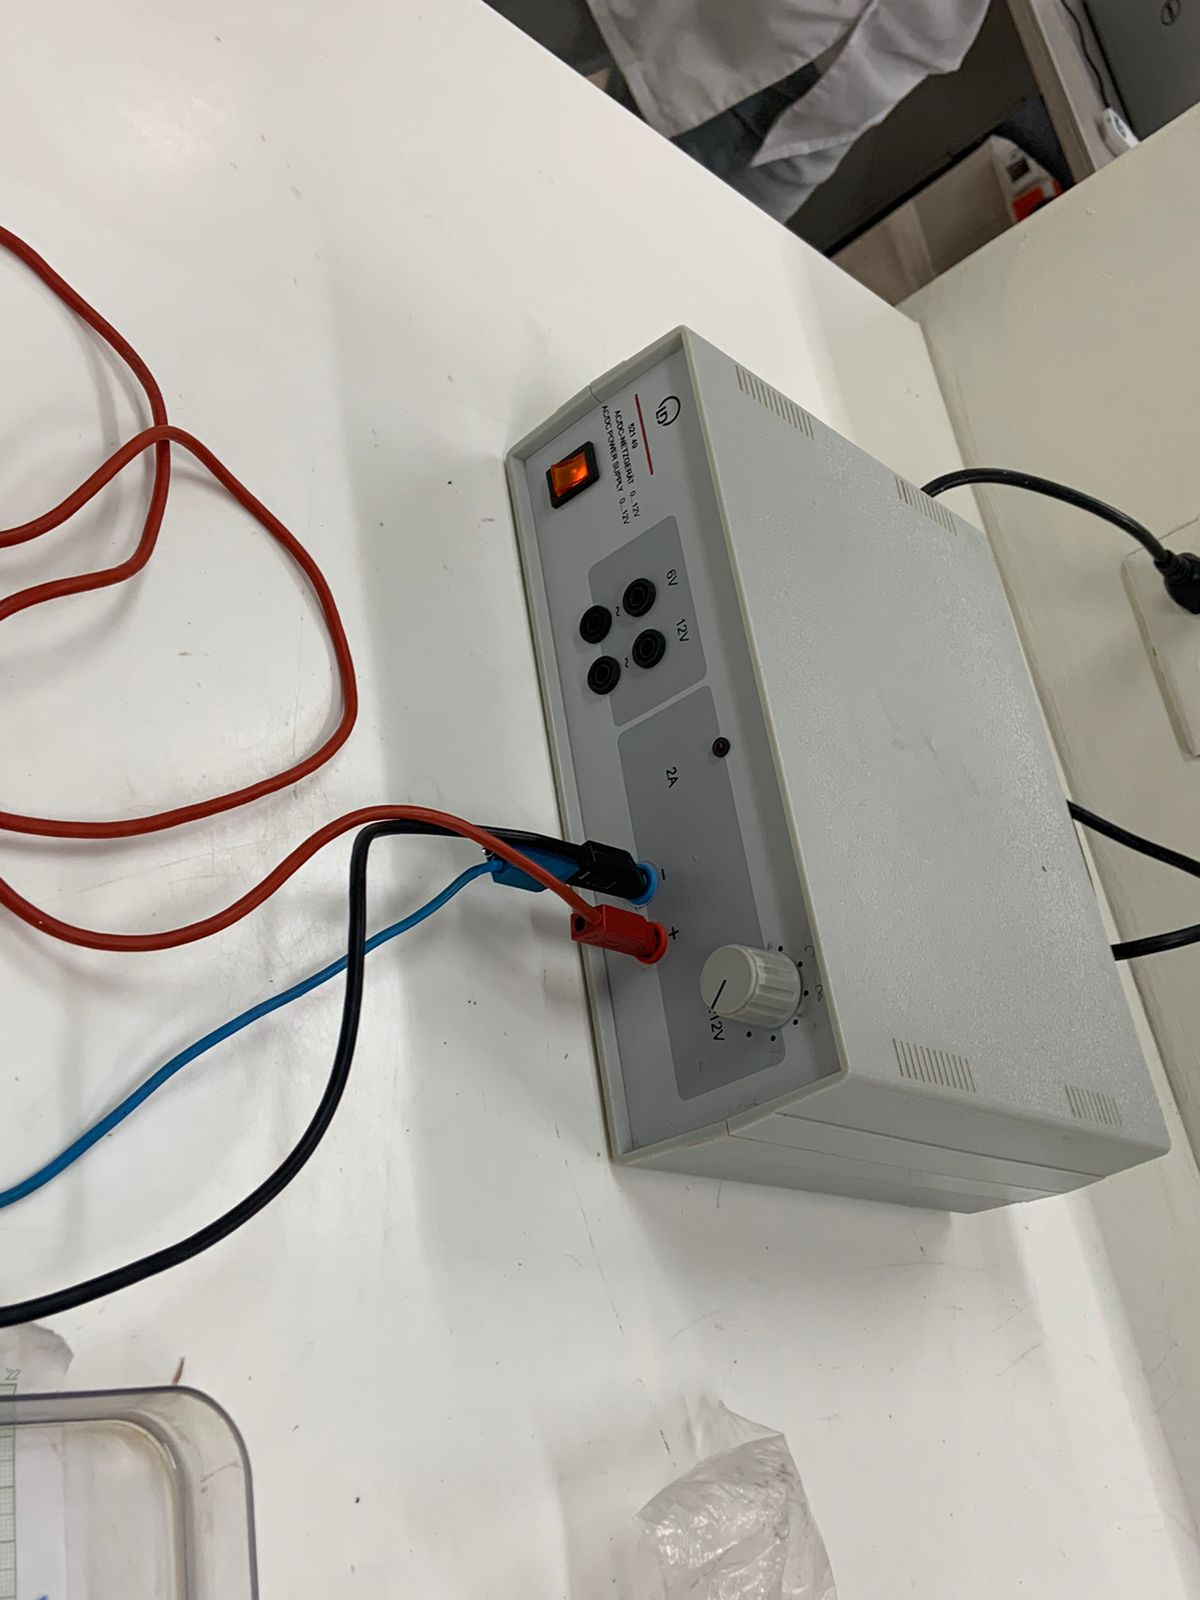
\includegraphics[scale = 0.3]{./Images/3.jpeg}
	\end{center}
\end{figure}

\begin{figure}[H]
	\begin{center}
		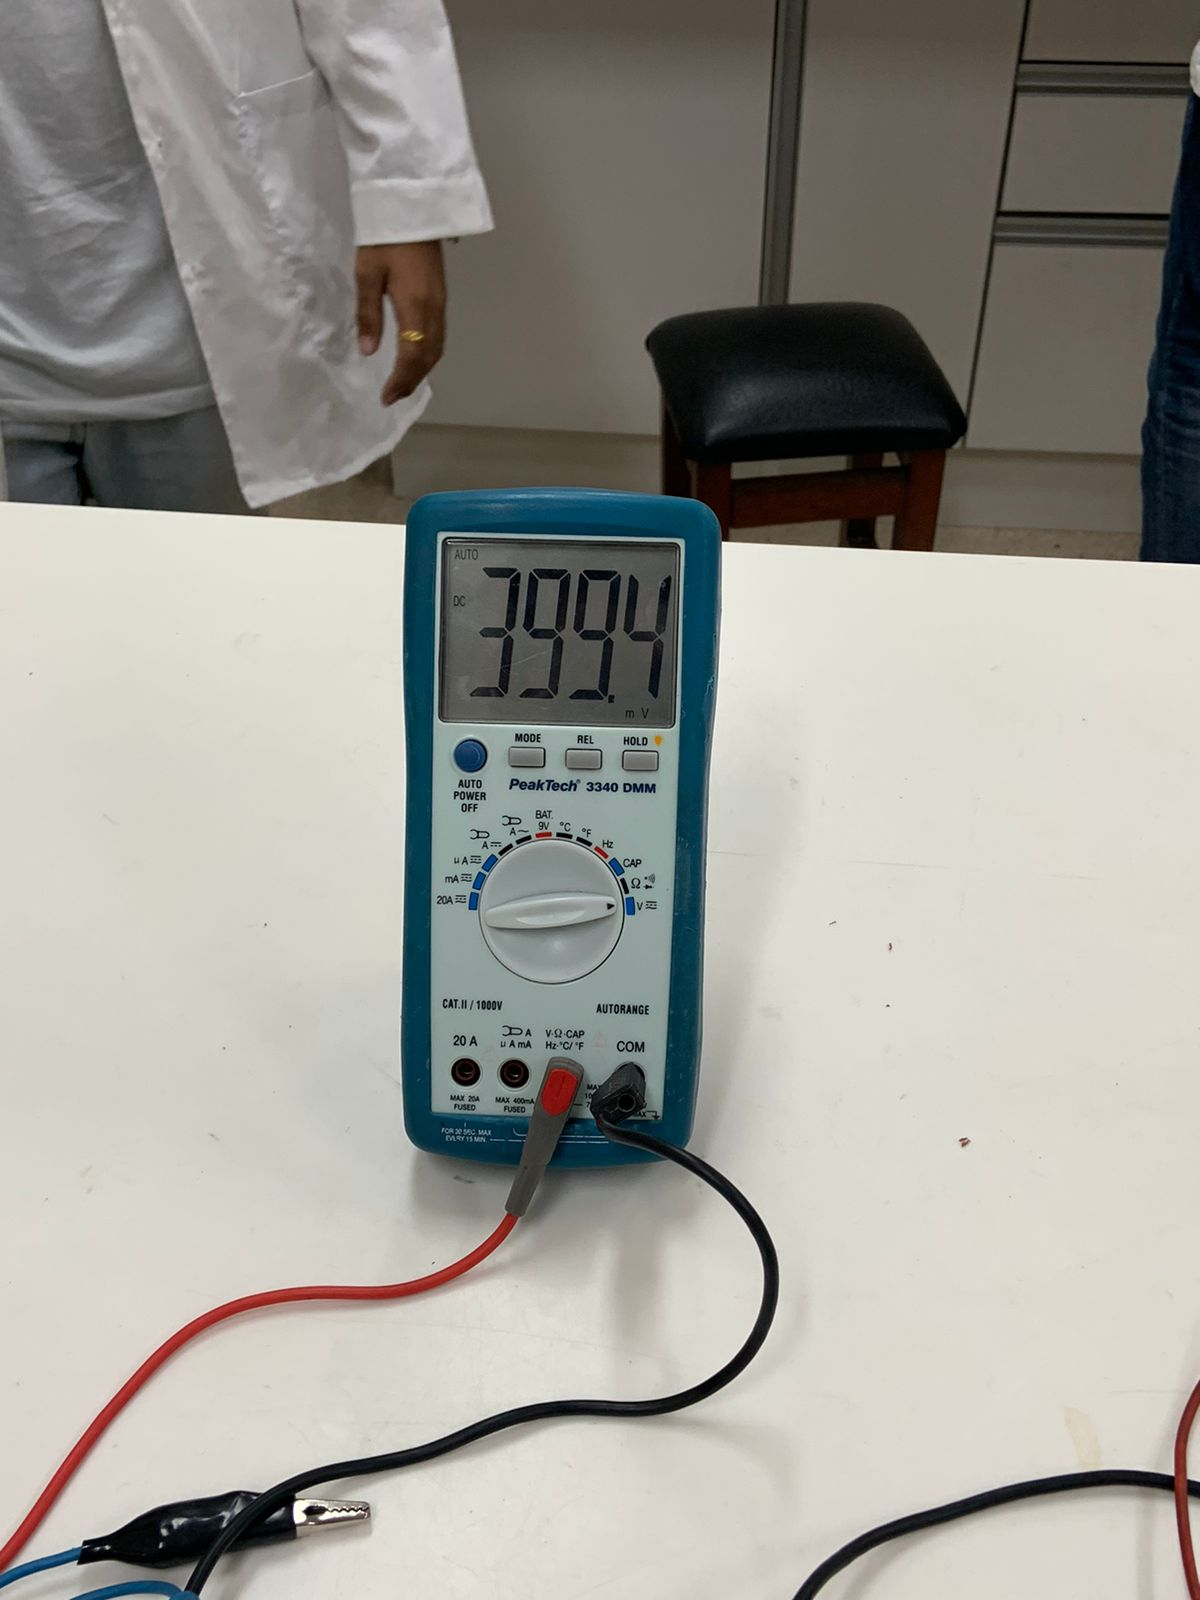
\includegraphics[scale = 0.3]{./Images/4.jpeg}
		\caption{Multímetro digital}
	\end{center}
\end{figure}

% ----------------------------------------------------------------------|>
\section{Datos Experimentales}

\begin{table}[H]
	\begin{center}
		% chktex-file 44
		\begin{tabular}{|p{2.5cm}|p{1.3cm}|p{2cm}|p{1.9cm}|p{1.9cm}|p{1.9cm}|p{1.9cm}|}

			% Table header

			Tipo         & Linea & $\triangle$V (V) &
			\multicolumn{4}{c}{Coordenadas (x,y)}                                              \\ \hline

			% 1st row {Paralelos} {1st V}

			Paralelo     & 1     & 4                & (-6.5,2)    & (-6.8,-4)   & (-4.2,10)  &
			(-3.6,-6.5)                                                                        \\

			% 2nd row
			             &
			             &
			             &
			(-3,3)       &
			(-4,-10.5)   &
			(-4.8,-13)   &
			(-4,-10.1)                                                                         \\ \hline

			% 1st row {Paralelos} {2nd V}

			Paralelo     & 2     & 6                & (1,2)       & (1.2,10.8)  & (1.2,-9.5) &
			(0.8,-1.8)                                                                         \\

			% 2nd row
			             &
			             &
			             &
			(-2.3,-5.5)  &
			(-2.5,-3)    &
			(1.3,-11.5)  &
			(1.4,-10)                                                                          \\ \hline

			% 1st row {Concéntricos} {1st V}

			Concéntricos & 3     & 4                & (-5,-4)     & (5.5,-4)    & (-6.5,-1)  &
			(-2.5,6.2)                                                                         \\

			% 2nd row
			             &
			             &
			             &
			(6.2,2.5)    &
			(-3.2,-5.9)  &
			(4,-5.5)     &
			(6.5,0.2)                                                                          \\ \hline

			% 1st row {Concéntricos} {1st V}

			Concéntricos & 4     & 6                & (-3.5,-4.5) & (4.6,3.1)   & (3,-4.2)   &
			(-1,5.7)                                                                           \\

			% 2nd row
			             &
			             &
			             &
			(-5.5,-1.4)  &
			(-3.8,4)     &
			(-5.5,0.5)   &
			(2.5,5.5)                                                                          \\ \hline

			% 1st row {Puntuales} {1st V}

			Puntuales    & 5     & 4                & (-4.5,4)    & (-8.3,11.3) & (-4,0.5)   &
			(-8.7,11.5)                                                                        \\

			% 2nd row
			             &
			             &
			             &
			(-6.1,-6.1)  &
			(-8,10.2)    &
			(-4.5,-2.8)  &
			(-7.8,8.5)                                                                         \\ \hline

			% 1st row {Puntuales} {2st V}

			Puntuales    & 6     & 6                & (-0.5,-0.5) & (-0.5,1)    & (-0.8,-4)  &
			(-0.8,-4)                                                                          \\

			% 2nd row
			             &
			             &
			             &
			(-7.2,8.2)   &
			(-0.8,-6.5)  &
			(0.8,1.8)    &
			(0.8,11.5)                                                                         \\ \hline
		\end{tabular}

	\end{center}
\end{table}

% ----------------------------------------------------------------------|>
\section{Análisis de datos}

% -----------------------|>
\subsection{Trazo de lineas de campo eléctrico}

\begin{figure}[H]
	\begin{center}
		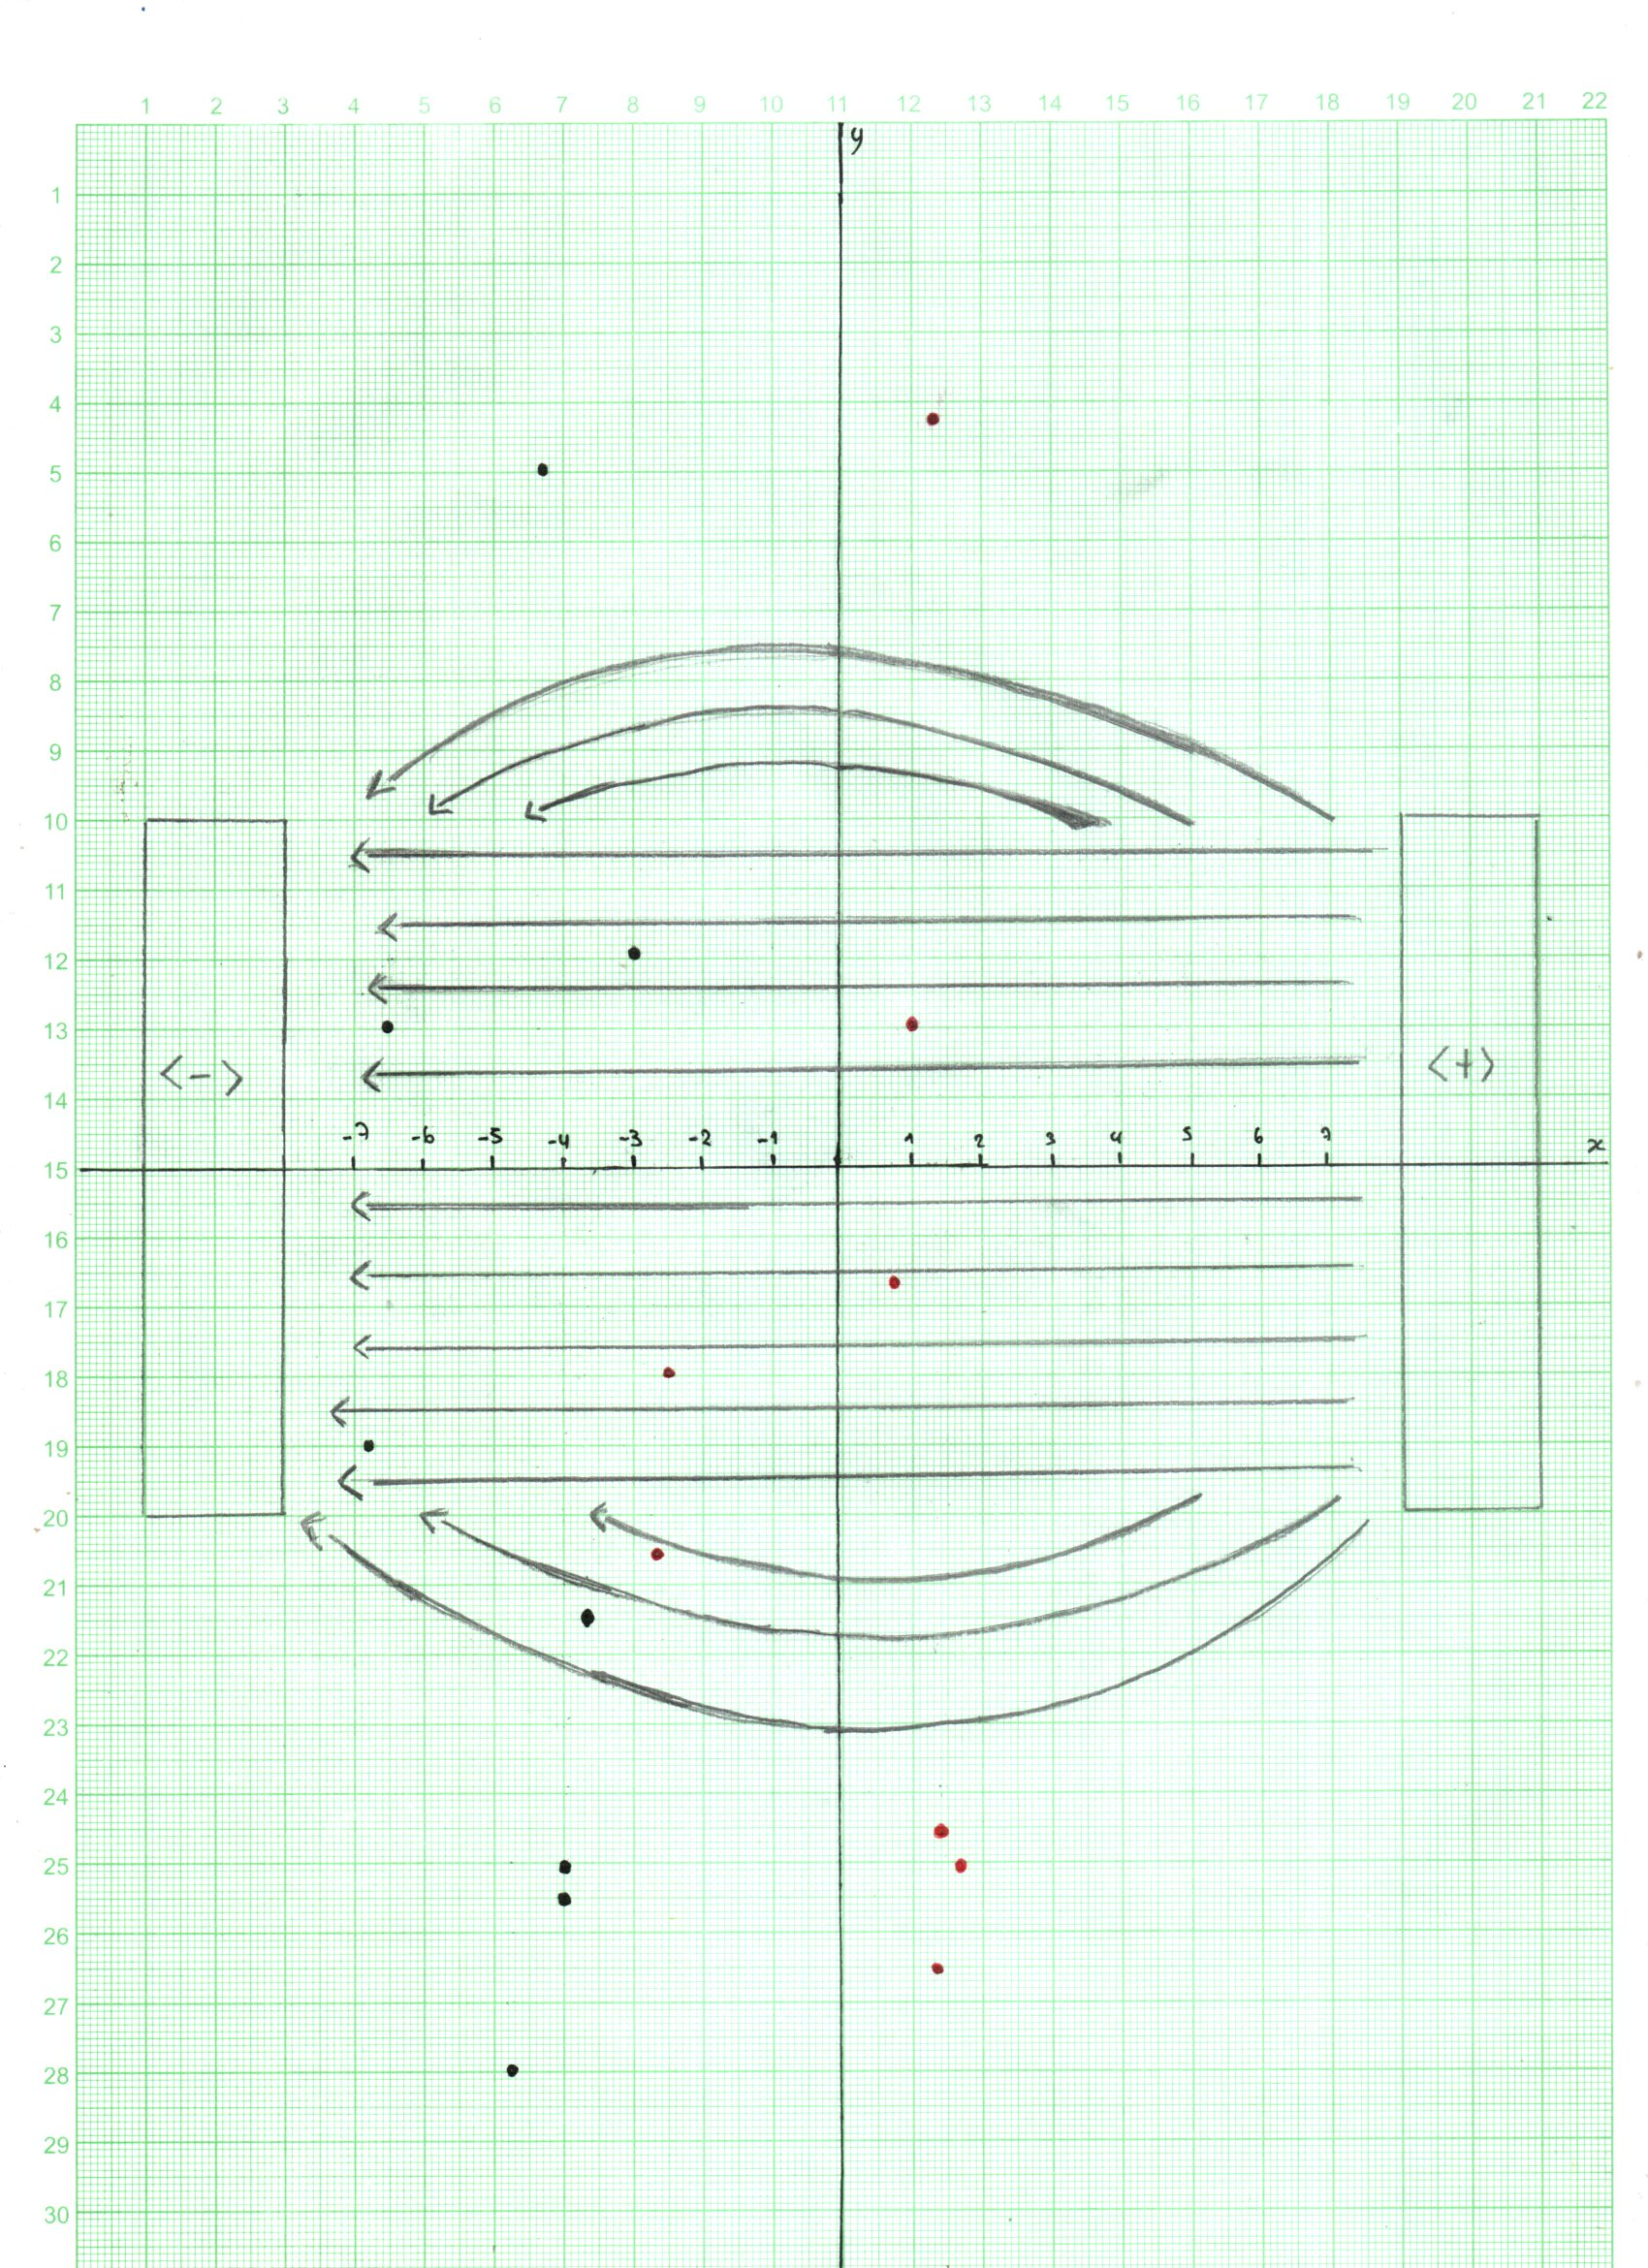
\includegraphics[scale = 0.6]{./Images/Paralelos.jpg}
		\caption{(A) Electrodos Paralelos}
	\end{center}
\end{figure}

\begin{figure}[H]
	\begin{center}
		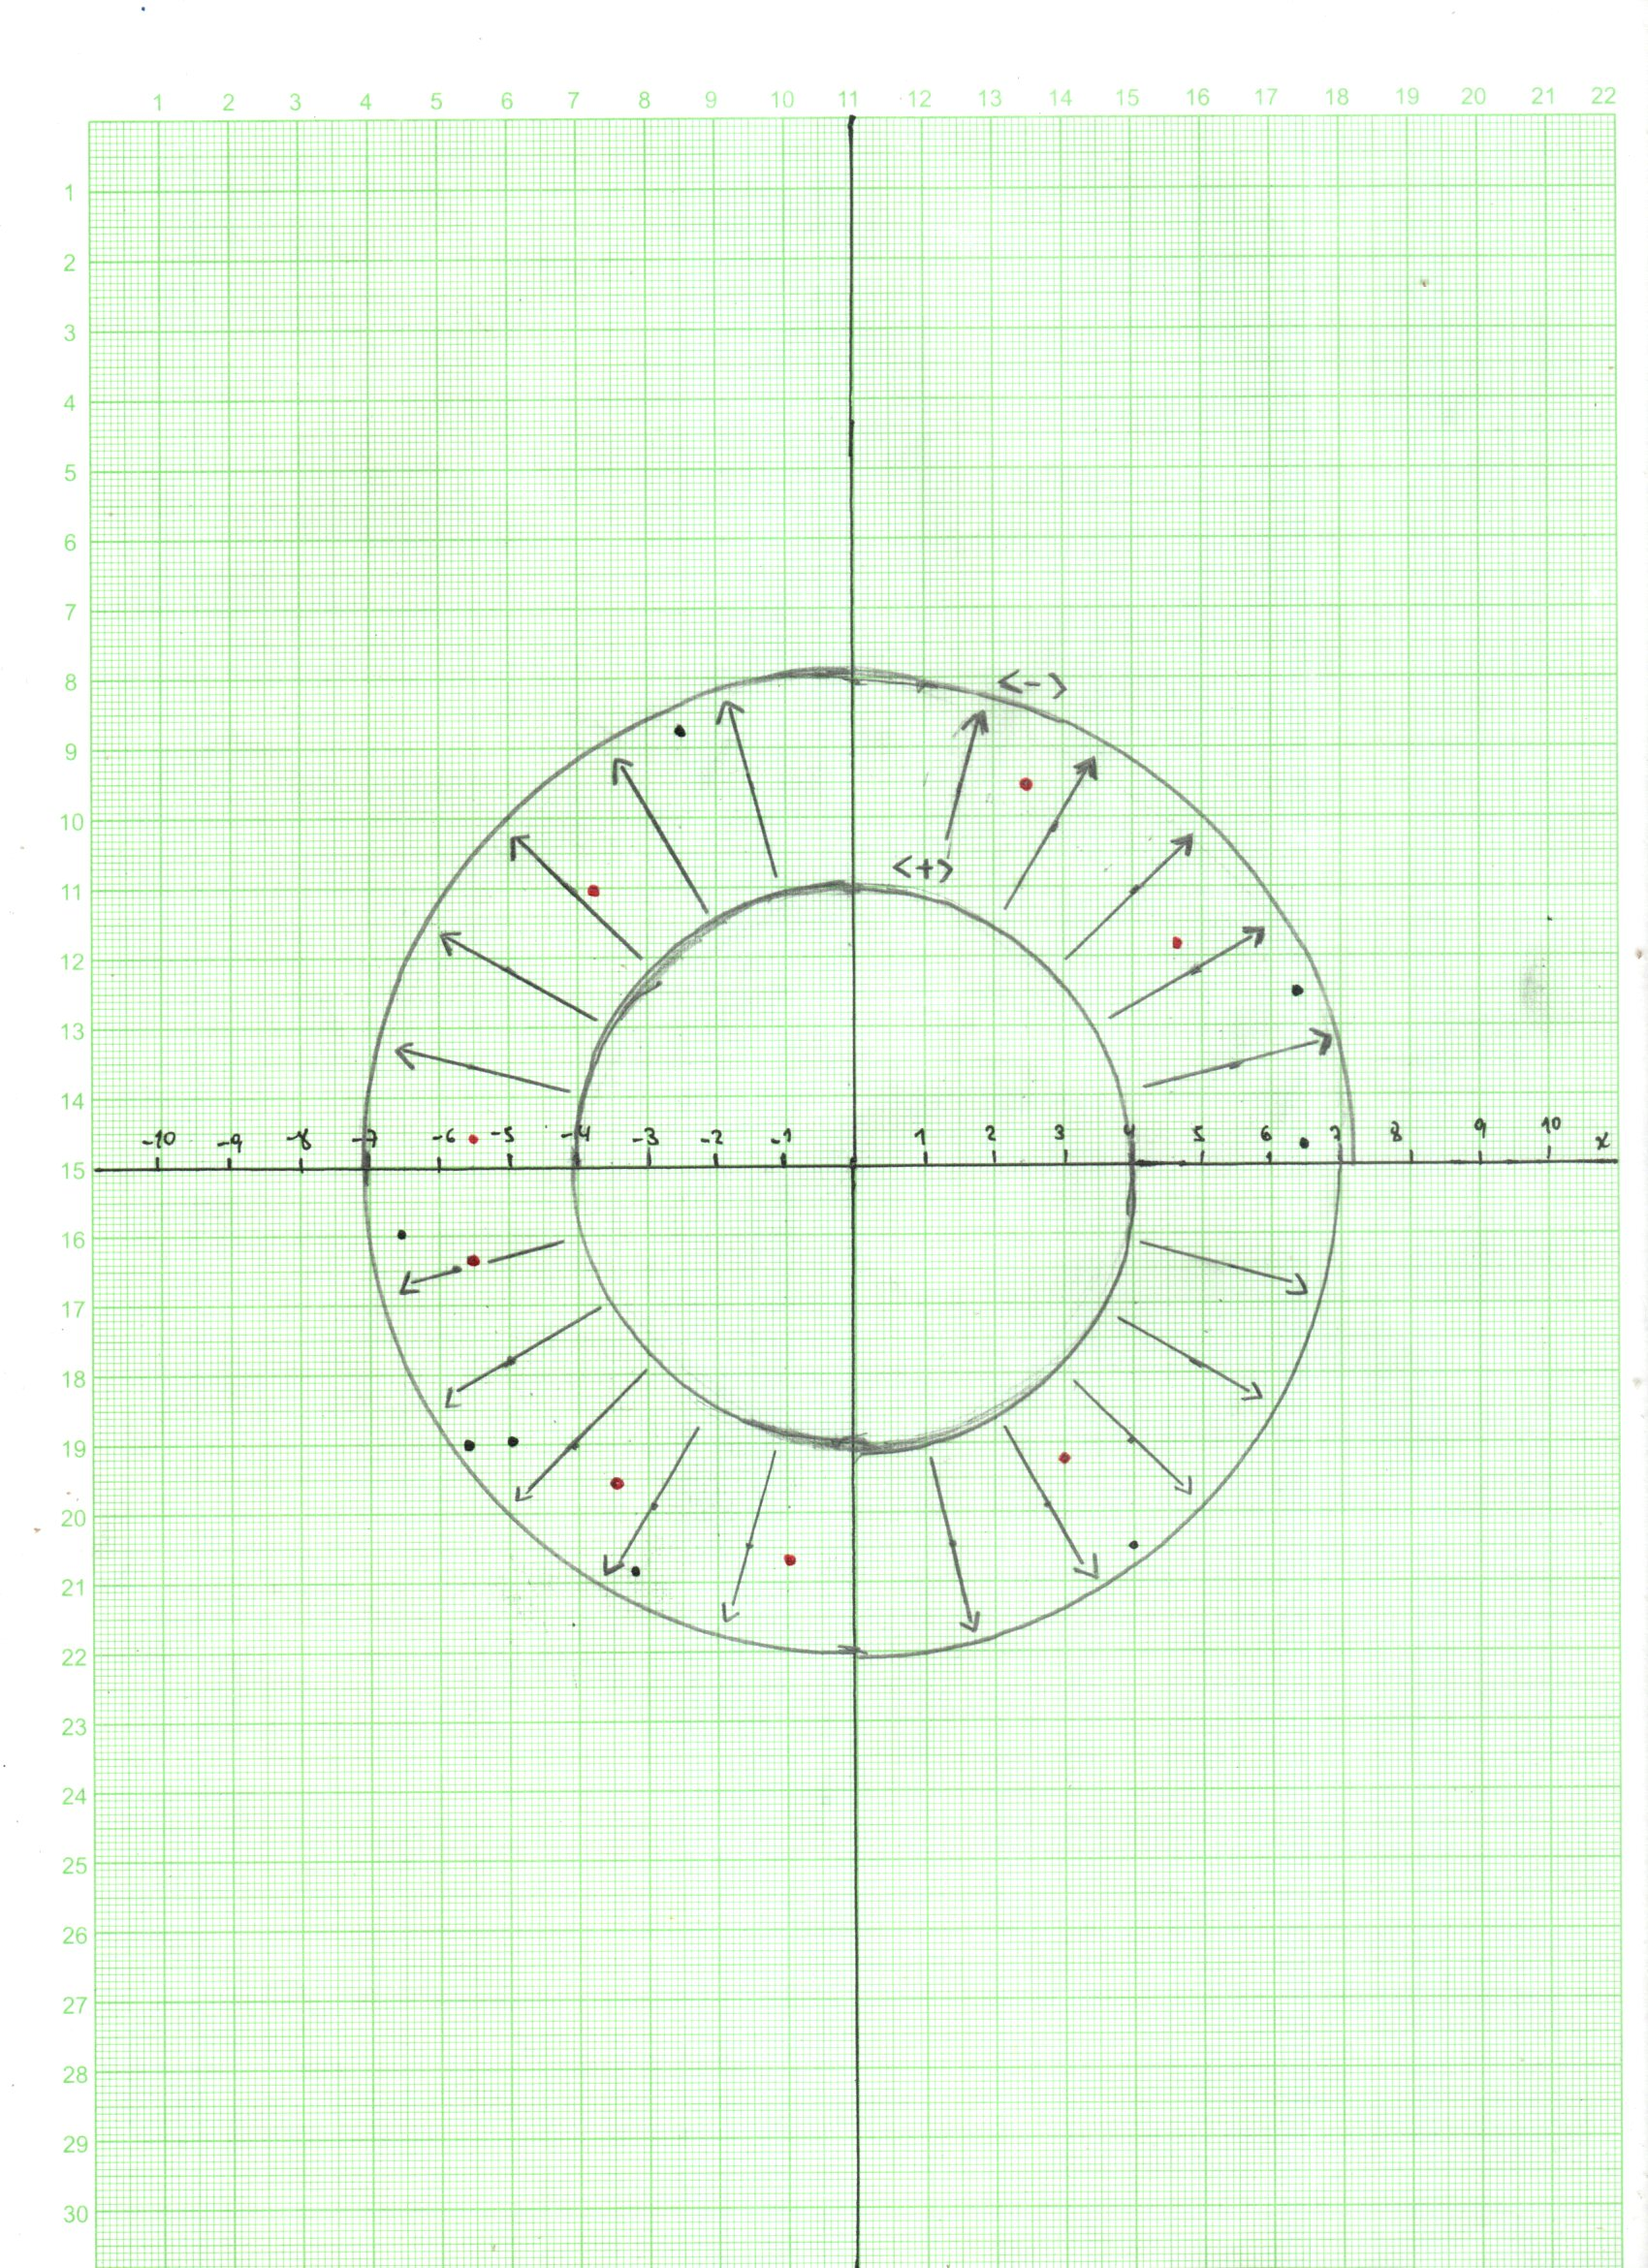
\includegraphics[scale = 0.75]{./Images/Concenctricos.jpg}
		\caption{(B) Electrodos Concéntricos}
	\end{center}
\end{figure}

\begin{figure}[H]
	\begin{center}
		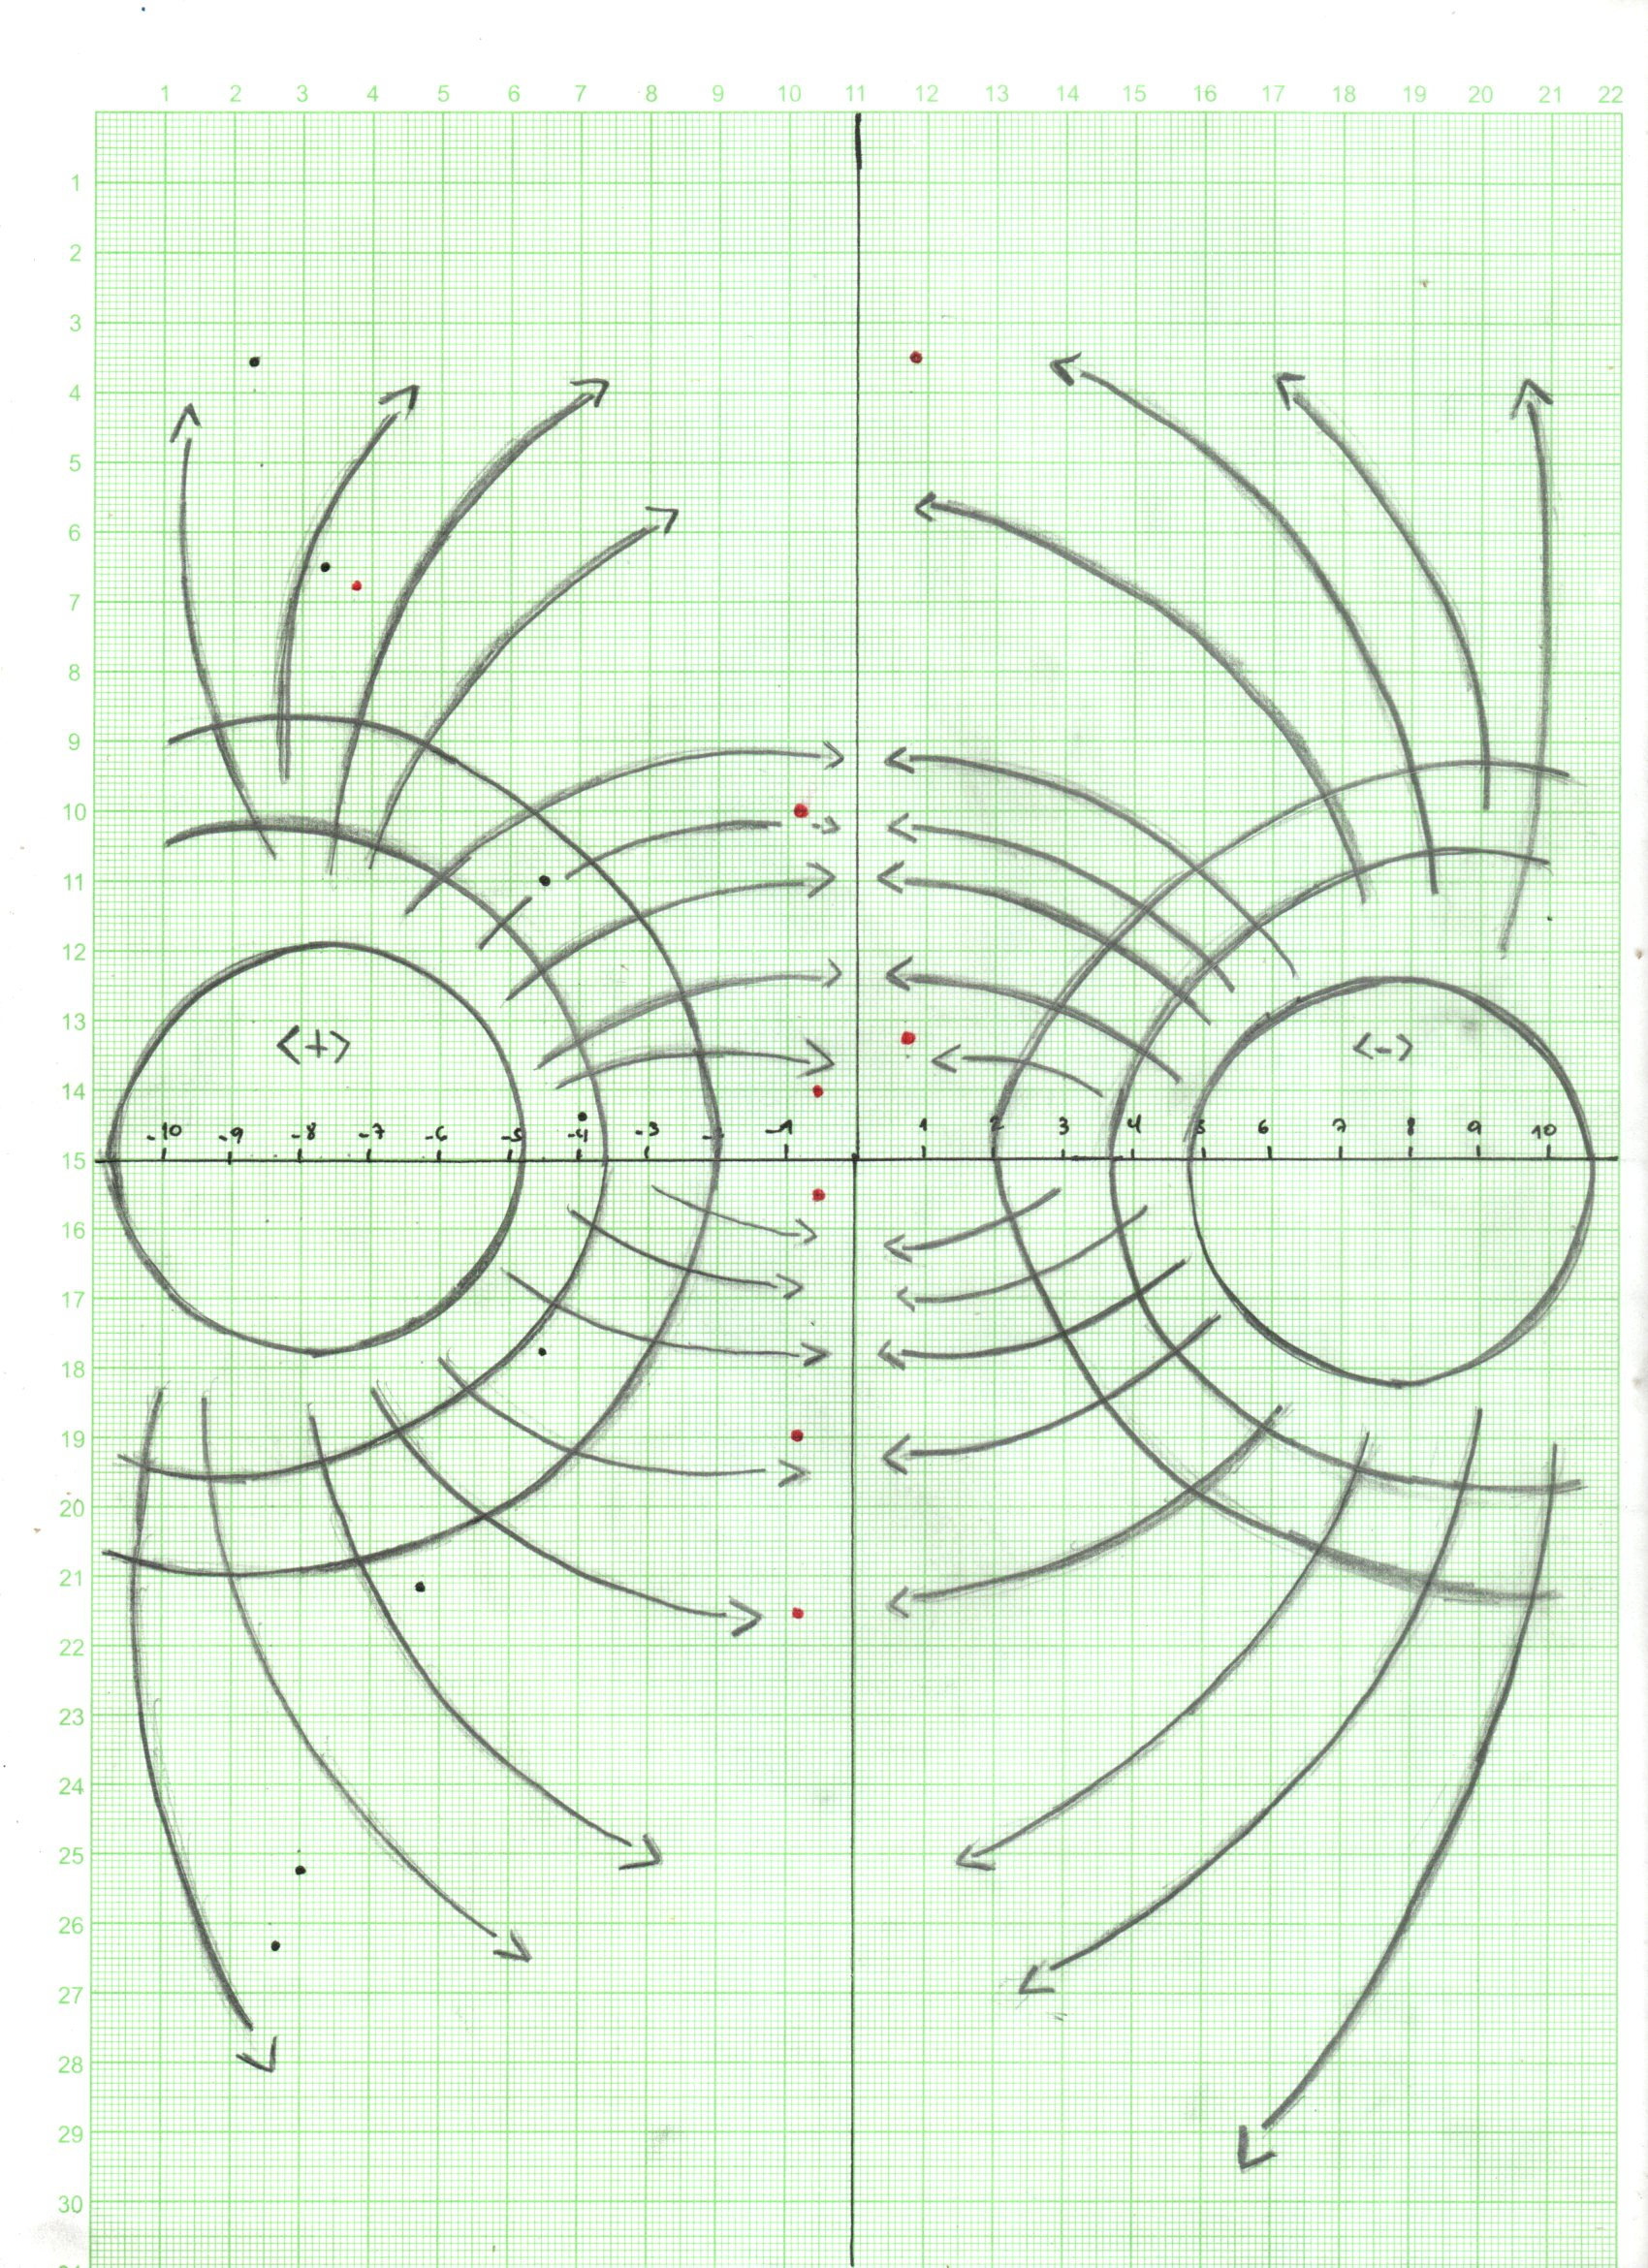
\includegraphics[scale = 0.7]{./Images/Puntuales.jpg}
		\caption{(C) Electrodos Puntuales}
	\end{center}
\end{figure}

% -----------------------|>
\subsection{Análisis de las lineas}

% -----------------------|>
\subsubsection{5. ¿Cuál fue el criterio que usted uso para trazar las líneas
	de campo eléctrico?}

Para trazar correctamente una línea de campo eléctrico, es
importante tener en cuenta que estas líneas nunca deben
interceptarse entre sí y deben incluir flechas que indiquen
su dirección y sentido en el campo.

% -----------------------|>
\subsubsection{6. ¿Cómo justifica la dirección de las líneas de campo
	eléctrico dibujadas?}

Cada carga positiva en un campo eléctrico tiene su
correspondiente carga negativa, y ambas cargas, junto con
sus coordenadas y voltajes, son utilizadas para crear una
simulación del campo. Las líneas de campo generadas son
simétricas a las cargas y proporcionales a su magnitud.

% -----------------------|>
\subsection{Análisis del campo en un punto}

% -----------------------|>
\subsubsection{7. ¿Cómo justifica la dirección del vector de campo eléctrico
	dibujado sobre el punto?}

La razón de esto se encuentra en la naturaleza de las
cargas, ya que las cargas positivas emanan del campo
mientras que las cargas negativas entran en él. Por lo
tanto, el vector que indica la dirección del campo seguirá
una trayectoria hacia la carga más cercana.

\subsubsection{8. ¿Por qué por un punto no deben pasar más de dos líneas
	de campo eléctrico?}

En un campo eléctrico, no debe haber más de dos líneas de
campo eléctrico que pasen por un mismo punto. Esto se debe
a que las líneas de campo eléctrico representan la
dirección del vector del campo eléctrico en un punto
determinado. Si hubiera más de dos líneas de campo que
pasaran por un punto, indicaría que hay diferentes vectores
de campo eléctrico en ese punto, lo cual no es posible ya
que el vector del campo eléctrico en un punto dado debe ser
único. Por lo tanto, para mantener la unicidad del vector
del campo eléctrico en un punto determinado, solo pueden
pasar dos líneas de campo eléctrico por ese punto.

% -----------------------|>
\subsection{Análisis de los electrodos puntuales de diferente signo}

% -----------------------|>
\subsubsection{9. ¿Cuál es el valor del potencial en el punto central de la
	línea que une los dos electrodos puntuales, medido respecto al electrodo
	negativo?}

En un punto central ubicado entre dos electrodos puntuales
con cargas iguales pero de signo opuesto, el valor del
voltaje es cero voltios. Esto se debe a que en este punto
los voltajes de ambas cargas son iguales, pero con signos
opuestos. Debido a que un voltaje es positivo y el otro es
negativo, se anulan entre sí, dando como resultado un
voltaje neto de cero.

% -----------------------|>
\subsubsection{10. ¿Cuál es el valor del potencial en el punto central de la
	línea que une los dos electrodos puntuales, medido respecto al electrodo
	positivo?}

Al ser cargas iguales, pero de signo contrario. Justo en
ese punto los voltajes son iguales para las dos cargas,
debido que al momento de ingresarlos en la formula de
potencial eléctrico, los valores se cancelan entre si,
ademas de tener la misma distancia el uno al otro.

% -----------------------|>
\subsubsection{11. ¿Cuál es el valor del potencial en tal punto central, medido
	respecto a un punto en el infinito donde el potencial es cero? Justifique
	su respuesta de acuerdo a la línea equipotencial que pasa por ese punto.}

\begin{figure}[H]
	\begin{center}
		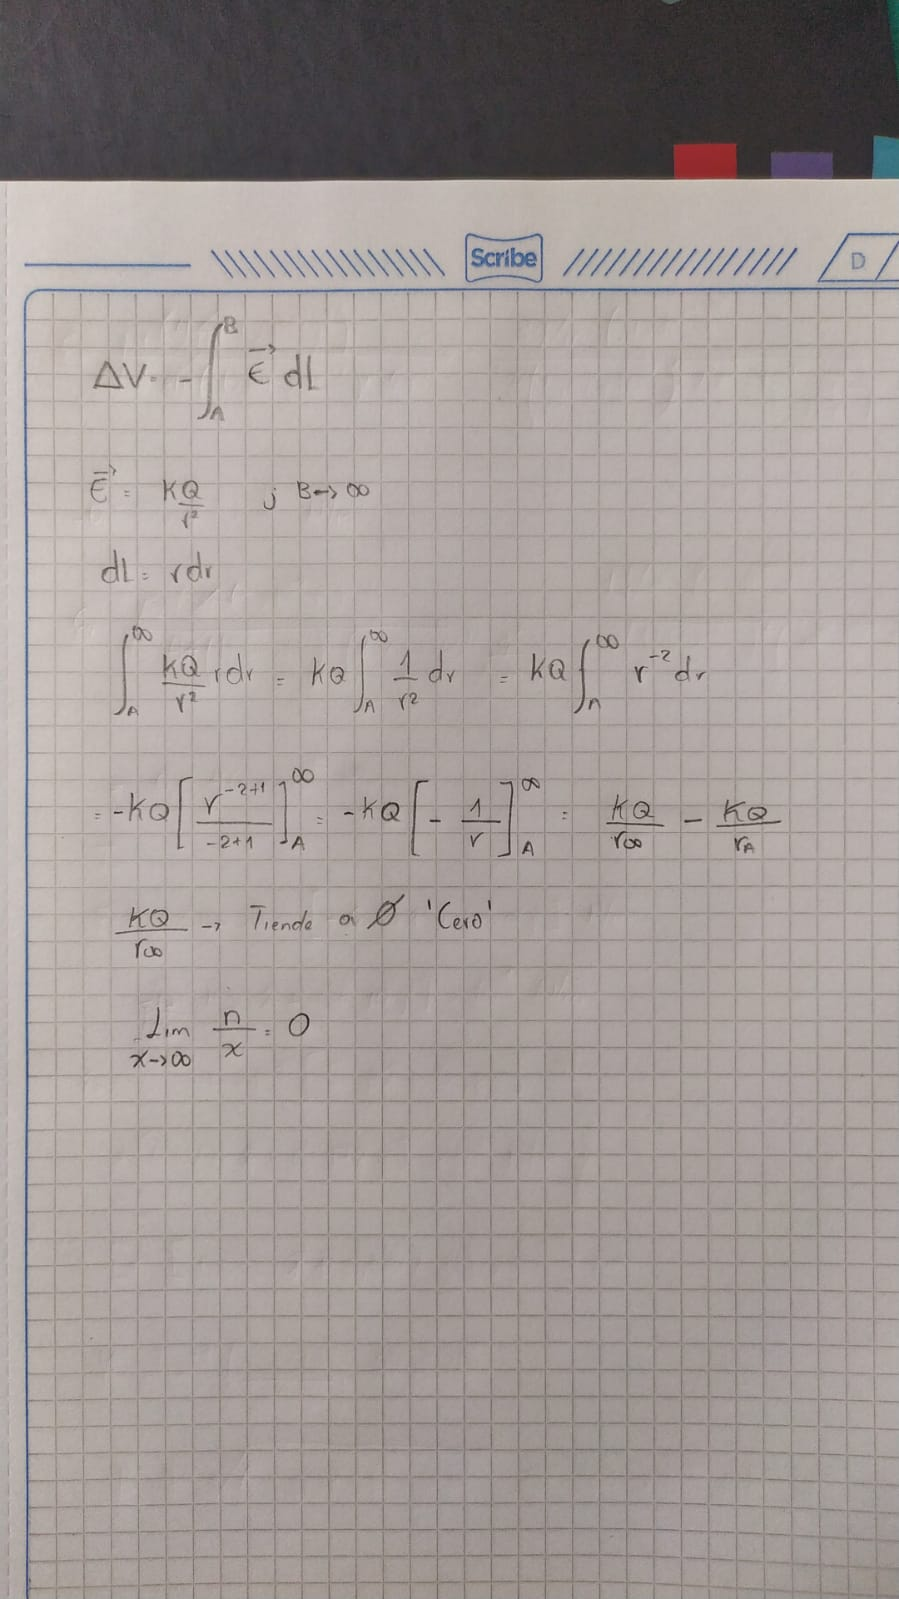
\includegraphics[scale = .4]{./Images/Proceso.jpeg}
	\end{center}
\end{figure}

% -----------------------|>
\subsection{Análisis de los electrodos puntuales de igual signo}

% -----------------------|>
\subsubsection{12. ¿Cuál es el valor del potencial en el punto central de la
	línea que une los dos electrodos puntuales, medido respecto al electrodo
	negativo?}

El potencial en la coordenada (0,0). Medido desde el electrodo negativo es 
0.025

% -----------------------|>
\subsubsection{13. ¿Cuál es el valor del potencial en el punto central de la
	línea que une los dos electrodos puntuales, medido respecto a uno de los
	electrodos positivos?}

El potencial en la coordenada (0,0). Medido desde el electrodo positivo es 
-0.025

% -----------------------|>
\subsubsection{14. ¿Cuál es el valor del campo eléctrico en ese punto?
	Justifique.}

En ese punto específico, el valor del campo eléctrico es
cero, ya que las cargas son de igual magnitud pero de
signos opuestos, lo que produce fuerzas de igual magnitud
pero con direcciones opuestas. Al sumar estas fuerzas, el
resultado es cero, lo que significa que el campo eléctrico
también es cero en ese punto

% -----------------------|>
\subsubsection{15. ¿Debe pasar alguna línea de campo eléctrico por ese punto
	central? Justifique}

Por el punto central no pasa ninguna cargas, debido a la naturaleza de las cargas
del mismo signo, estas no pueden tocarse, por lo que se crea una asíntota
vertical entre ellas.

% -----------------------|>
\subsection*{Análisis de electrodos concéntricos}

% -----------------------|>
\subsubsection{16. Realice una gráfica de diferencia de potencial ($\triangle$V)
	en puntos dentro del anillo exterior contra la distancia (r) medida desde el centro}

\subsubsection*{Para 4V:\@(Usando la formula de distancia entre puntos)}

\begin{figure}[H]
	\begin{center}
		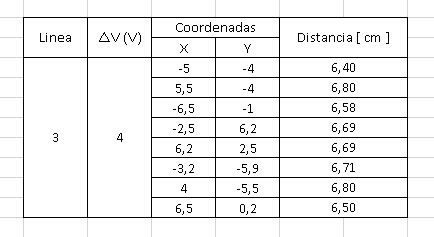
\includegraphics[scale = 1]{./Images/Concentricos1.png}
	\end{center}
\end{figure}

\subsubsection*{Para 6V:\@(Usando la formula de distancia entre puntos)}

\begin{figure}[H]
	\begin{center}
		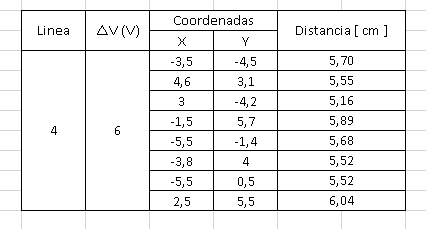
\includegraphics[scale = 1]{./Images/Concentricos2.PNG}
	\end{center}
\end{figure}

% -----------------------|>
\subsubsection{17. ¿En qué región la diferencia de potencial es constante? ¿Por qué es de esperar que
	sea constante en esa región?}

A fin de que se mantenga una diferencia de potencial constante, es 
importante que su valor permanezca invariable en cualquier punto 
seleccionado. Es necesario mantener esta constancia de la diferencia 
de potencial en las áreas de interés, incluyendo las zonas entre los 
electrodos positivos y la región externa de la esfera concéntrica.

% -----------------------|>
\subsubsection{18. ¿Qué valor toma el campo eléctrico dentro de esa región?}

En la zona en cuestión, el campo eléctrico tiene un valor de cero N/c en 
ambas caras, ya que en la región interna no hay cargas encerradas y su valor 
es nulo. Además, en la región externa, el campo generado por la esfera negativa 
anula el campo generado por la esfera cargada negativamente, lo que resulta 
en un valor neto de campo eléctrico igual a cero.

% ----------------------------------------------------------------------|>
\section{Conclusiones}

En el informe presentado se puede analizar algunas de las 
características que presentan las líneas de campo eléctrico 
y las líneas equipotenciales, a su vez fue posible evidenciar 
la relación que tienen estas dos, ya que son perpendiculares 
entre ellas. Mediante la experimentación se notó la importancia
 de tener un punto de referencia especifico para obtener la 
 medida de potencial eléctrico requerida; es decir, si 
 ubicamos el eje de referencia en distintos puntos 
 (ya se más cerca o más lejos de una de las cargas), 
 será diferente la medida del potencial eléctrico; 
 de igual forma cuando tenemos en un punto un potencial 
 eléctrico cero, su campo eléctrico también lo será.
Cuando trabajamos con superficies equipotenciales, los 
movimientos realizados a lo largo de la superficie no 
representan el trabajo realizado, esto quiere decir que 
no hay trabajo, ya que el movimiento realizado es 
perpendicular al campo eléctrico.

\newpage

\bibliography{./Bibliography/bibliography.bib}

\end{document}